\ifx\wholebook\relax \else

\documentclass{article}

%
% loading packages
%

\RequirePackage{ifpdf}
\RequirePackage{ifxetex}

%
%
\ifpdf
  \RequirePackage[pdftex,%
       bookmarksnumbered,%
              colorlinks,%
          linkcolor=blue,%
              hyperindex,%
        plainpages=false,%
       pdfstartview=FitH]{hyperref}
\else\ifxetex
  \RequirePackage[bookmarksnumbered,%
               colorlinks,%
           linkcolor=blue,%
               hyperindex,%
         plainpages=false,%
        pdfstartview=FitH]{hyperref}
\else
  \RequirePackage[dvipdfm,%
        bookmarksnumbered,%
               colorlinks,%
           linkcolor=blue,%
               hyperindex,%
         plainpages=false,%
        pdfstartview=FitH]{hyperref}
\fi\fi
%\usepackage{hyperref}

% other packages
%--------------------------------------------------------------------------
\usepackage{graphicx, color}
\usepackage{wrapfig}
\usepackage{subfig}
\usepackage{multicol}
\usepackage{tikz}
\usetikzlibrary{matrix,positioning,shapes}
\usetikzlibrary{patterns}

\usepackage{amsmath, amsthm, amssymb} % for math
\usepackage{exercise} % for exercise
\usepackage{import} % for nested input

%
% for programming
%
\usepackage{verbatim}
\usepackage{fancyvrb}
\usepackage{listings}
%\usepackage{algorithmic} %old version; we can use algorithmicx instead
%\usepackage[plain]{algorithm} %remove rule (horizontal line on top/below the algorithm
\usepackage{algorithm} %to remove rules change to \usepackage[plain]{algorithm}
%\usepackage{algorithm2e}
\usepackage[noend]{algpseudocode} %for pseudo code, include algorithmicsx automatically
\usepackage{appendix}
\usepackage{makeidx} % for index support
\usepackage{titlesec}
\usepackage{epigraph}

\usepackage[cm-default]{fontspec}
\usepackage{xunicode}
%\usepackage{fontenc}
\usepackage{textcomp}
\usepackage{url}

% detect and select Chinese font
% ------------------------------
% fc-list :lang=zh    % list all Chinese fonts
% fc-list :mono       % list all mono fonts
% fc-cache            % refresh cache to load new installed fonts
\def\macmainfont{STSong}  % Under Mac OS X
\def\macmonofont{Monaco}
\def\winmainfont{SimSun} % Under Windows
\def\winmonofont{Consolas}
\def\linuxmainfont{WenQuanYi Micro Hei} % Under Linux
\def\linuxmainfont{Courier}

\suppressfontnotfounderror1 % Avoid setting exit code (error level) to break make process
\count255=\interactionmode
\batchmode

% main font
\let\mainft=\macmainfont
\font\thefont="\mainft"\space at 10pt
\ifx\thefont\nullfont
  \let\mainft=\winmainfont
  \font\thefont="\mainft"\space at 10pt
  \ifx\the\nullfont
    \let\mainft=\linuxmainfont
    \font\thefont="\mainft"\space at 10pt
    \ifx\the\nullfont
      \errorstopmode
      \errmessage{no suitable Chinese main font found}
    \fi
  \fi
\fi

% mono font
\let\monoft=\macmonofont
\font\thefont="\monoft"\space at 10pt
\ifx\thefont\nullfont
  \let\monoft=\winmonofont
  \font\thefont="\monoft"\space at 10pt
  \ifx\the\nullfont
    \let\monoft=\linuxmonofont
    \font\thefont="\monoft"\space at 10pt
    \ifx\the\nullfont
      \errorstopmode
      \errmessage{no suitable mono font found}
    \fi
  \fi
\fi

\interactionmode=\count255

\setmainfont[Mapping=tex-text]{\mainft}
\setmonofont[Scale=MatchLowercase]{\monoft}   % 英文等宽字体

\XeTeXlinebreaklocale "zh"  % to solve the line breaking issue
\XeTeXlinebreakskip = 0pt plus 1pt minus 0.1pt

\titleformat{\paragraph}
{\normalfont\normalsize\bfseries}{\theparagraph}{1em}{}
\titlespacing*{\paragraph}
{0pt}{3.25ex plus 1ex minus .2ex}{1.5ex plus .2ex}

\lstdefinelanguage{Smalltalk}{
  morekeywords={self,super,true,false,nil,thisContext}, % This is overkill
  morestring=[d]',
  morecomment=[s]{"}{"},
  alsoletter={\#:},
  escapechar={!},
  literate=
    {BANG}{!}1
    {UNDERSCORE}{\_}1
    {\\st}{Smalltalk}9 % convenience -- in case \st occurs in code
    % {'}{{\textquotesingle}}1 % replaced by upquote=true in \lstset
    {_}{{$\leftarrow$}}1
    {>>>}{{\sep}}1
    {^}{{$\uparrow$}}1
    {~}{{$\sim$}}1
    {-}{{\sf -\hspace{-0.13em}-}}1  % the goal is to make - the same width as +
    %{+}{\raisebox{0.08ex}{+}}1		% and to raise + off the baseline to match -
    {-->}{{\quad$\longrightarrow$\quad}}3
	, % Don't forget the comma at the end!
  tabsize=2
}[keywords,comments,strings]

% for literate Haskell code
\lstdefinestyle{Haskell}{
  flexiblecolumns=false,
  basewidth={0.5em,0.45em},
  morecomment=[l]--,
  literate={+}{{$+$}}1 {/}{{$/$}}1 {*}{{$*$}}1 {=}{{$=$}}1
           {>}{{$>$}}1 {<}{{$<$}}1 {\\}{{$\lambda$}}1
           {\\\\}{{\char`\\\char`\\}}1
           {->}{{$\rightarrow$}}2 {>=}{{$\geq$}}2 {<-}{{$\leftarrow$}}2
           {<=}{{$\leq$}}2 {=>}{{$\Rightarrow$}}2
           {\ .}{{$\circ$}}2 {\ .\ }{{$\circ$}}2
           {>>}{{>>}}2 {>>=}{{>>=}}2
           {|}{{$\mid$}}1
}

% "define" Scala
\lstdefinelanguage{Scala}{
  morekeywords={abstract,case,catch,class,def,%
    do,else,extends,false,final,finally,%
    for,if,implicit,import,match,mixin,%
    new,null,object,override,package,%
    private,protected,requires,return,sealed,%
    super,this,throw,trait,true,try,%
    type,val,var,while,with,yield},
  otherkeywords={=>,<-,<\%,<:,>:,\#,@},
  sensitive=true,
  morecomment=[l]{//},
  morecomment=[n]{/*}{*/},
  morestring=[b]",
  morestring=[b]',
  morestring=[b]"""
}

\lstloadlanguages{C, C++, Java, Lisp, Haskell, Python, Smalltalk, Scala}

\lstset{
  basicstyle=\small\ttfamily,
  commentstyle=\rmfamily,
  texcl=true,
  showstringspaces = false,
  upquote=true,
  flexiblecolumns=false
}

\newcommand\doubleplus{+\kern-1.3ex+\kern0.8ex}

% ======================================================================

\def\BibTeX{{\rm B\kern-.05em{\sc i\kern-.025em b}\kern-.08em
    T\kern-.1667em\lower.7ex\hbox{E}\kern-.125emX}}

%
% mathematics
%
\newcommand{\be}{\begin{equation}}
\newcommand{\ee}{\end{equation}}
\newcommand{\bmat}[1]{\left( \begin{array}{#1} }
\newcommand{\emat}{\end{array} \right) }
\newcommand{\VEC}[1]{\mbox{\boldmath $#1$}}

% numbered equation array
\newcommand{\bea}{\begin{eqnarray}}
\newcommand{\eea}{\end{eqnarray}}

% equation array not numbered
\newcommand{\bean}{\begin{eqnarray*}}
\newcommand{\eean}{\end{eqnarray*}}

\newtheorem{theorem}{定理}[section]
\newtheorem{lemma}[theorem]{引理}
\newtheorem{proposition}[theorem]{Proposition}
\newtheorem{corollary}[theorem]{Corollary}

% 中文书籍设置
% ====================================
\renewcommand\contentsname{目\ 录}
%\renewcommand\listfigurename{插图目录}
%\renewcommand\listtablename{表格目录}
\renewcommand\figurename{图}
\renewcommand\tablename{表}
\renewcommand\proofname{证明}
\renewcommand\ExerciseName{练习}
%\renewcommand{\algorithmcfname}{算法}

\ifx\wholebook\relax
\renewcommand\bibname{参\ 考\ 文\ 献}                    %book类型
%\newtheorem{Definition}[Theorem]{定义}
\newtheorem{Theorem}{定理}[chapter]
\newtheorem{example}{例题}[chapter]
\else
\renewcommand\refname{参\ 考\ 文\ 献}
\fi

%\setcounter{secnumdepth}{4}
\titleformat{\chapter}
  {\normalfont\bfseries\Large}
  {第\arabic{chapter}章}
  {12pt}{\Large}
%% \titleformat{\subsection}
%%   {\normalfont\bfseries\large}
%%   {\CJKnumber{\arabic{subsection}}、}
%%   {12pt}{\large}
%% \titleformat{\subsubsection}
%%   {\normalfont\bfseries\normalsize}
%%   {\arabic{subsubsection}.}
%%   {12pt}{\normalsize}

%\renewcommand{\baselinestretch}{1.5}                        %文章行间距为1.5倍。

\makeatletter
\newcommand{\verbatimfont}[1]{\renewcommand{\verbatim@font}{\ttfamily#1}}
\makeatother

\setcounter{tocdepth}{4}
\setcounter{secnumdepth}{4}

%\verbatimfont{\footnotesize}


\setcounter{page}{1}

\begin{document}

\title{范畴论}

\author{刘新宇
\thanks{{\bfseries 刘新宇} \newline
  Email: liuxinyu95@gmail.com \newline}
  }

\maketitle
\fi

\markboth{范畴论}{编程的数学原理}

\ifx\wholebook\relax
\chapter{范畴论}
\numberwithin{Exercise}{chapter}
\fi

\epigraph{数学是赋予不同事物相同名字的艺术。}{——昂利$\cdot$庞加莱}

% Mathematics is the art of giving the same name to different things.

如果你已经坚持看到了本书这一章,我建议你小小的奖励自己一下。你已经迈过了第一道门槛,正在通往神奇的抽象王国之路上。这条路是世界上许多最聪明的心智披荆斩棘开辟出来的。如果说,人们将具体的事物,抽象成不带具体意义的数与形是原始阶段;将数、形与计算的意义去除,抽象成代数结构(例如群)和代数关系(例如同构)是第一阶段;范畴论可以算是抽象的第二阶段。

你也许会问,我们为什么要了解范畴论?这和编程有什么关系?对此有一个比较短的答案和一个比较长的答案。较短的回答是,如果不了解范畴论,过不了多久,你也许看不懂别人写的程序了。2010年以后,如果翻看Haskell标准库的源代码,就会发现几乎所有的内容,都用范畴论重新写过了。映射、叠加、遍历……几乎所有的计算都在说着范畴的语言,犹如天书。你也许觉得叠加操作可以这样写:

\lstset{language=Haskell, frame=single}
 \begin{lstlisting}
foldr _ z [] = z
foldr f z (x:xs) = f x (foldr f z xs)
\end{lstlisting}

实际上,今天的标准库用范畴的语言这样写:

\begin{lstlisting}
foldr f z t = appEndo (foldMap (Endo #. f) t) z
foldMap f = foldr (mappend . f) mempty
\end{lstlisting}

你也许觉得,反正工作中不用Haskell,不了解范畴论也没有关系。但是最近十几年的情况是,范畴论由于其强大的抽象,几乎普适于任何问题,正向其他的语言和环境中渗透。不要说各大编程语言纷纷引入lambda演算和闭包等结构,有超过20种语言已经实现了单子\cite{Monad-Haskell-Wiki}——用范畴论的语言说,叫做“函子范畴上的幺半群”。

较长的答案是:我们需要抽象。请原谅这个答案看起来更短。赫尔曼$\cdot$外尔说现代数学在过去几十年不断沉湎在抽象和形式化上。编程领域何尝不是如此呢?现代计算机科学解决的问题空前复杂,大数据量、分布式、高并发、还要保证数据和计算的安全。仅仅靠着前几十年的传统方法——暴力求解、务实的工程实践再加上一点聪明的头脑已经不够了。这逼迫着我们去吸取其他科学和数学中的新方法和新工具。

正如迪厄多内所说:“这种抽象绝不是来自数学家的反常意愿,似乎他们想通过使用深奥莫测的语言来把自己与其它人隔开。数学家是被经典对象和关系的本质特性逼着去锻造新的抽象工具,来解决过去看来是不可攻克的问题。”\cite{Dieudonne1987}

本章内容将再次挑战我们的抽象思维。如果读完一遍没有理解是完全正常的。请不要灰心丧气,生活不是直线发展的,我们理解知识的过程是螺旋上升的。要不断回过头去反复体会。开卷有益,去阅读大师的作品。也许某个瞬间豁然开朗,就能体会到“蓦然回首,那人却在灯火阑珊处”的感觉。

范畴论是数学家艾伦伯格和麦克兰恩在1940年代创立的。

\begin{wrapfigure}{R}{0.3\textwidth}
 \centering
 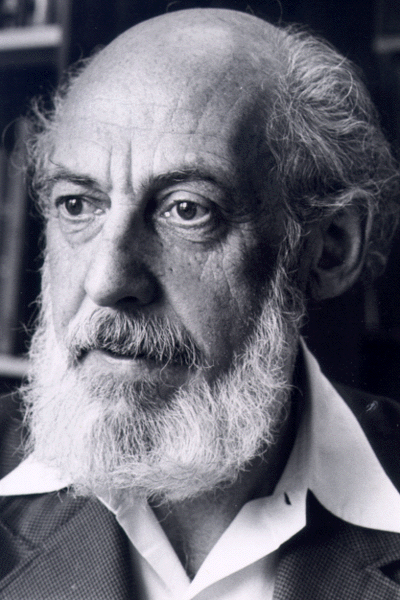
\includegraphics[scale=0.25]{img/Eilenberg.eps}
 \captionsetup{labelformat=empty}
 \caption{艾伦伯格(Samuel Eilenberg, 1913 - 1998)}
 \label{fig:Eilenberg}
\end{wrapfigure}

塞缪尔·艾伦伯格于1913年生于波兰华沙的一个犹太人家庭。他于1936年在华沙大学获得博士学位。艾伦伯格主要研究代数拓扑。他与诺曼·斯廷罗德(Norman Steenrod)一起对同调理论进行了公理化。艾伦伯格在与麦克兰恩合作研究同调代数的过程中一起创立了范畴论。艾伦伯格也是著名的布尔巴基小组成员。他与昂利·嘉当合作,在1956年完成了经典著作《同调代数》。艾伦伯格后来移居美国,在纽约哥伦比亚大学做教授,他的主要工作是发展纯粹的范畴论,是该领域的奠基者之一。1986年他获得沃尔夫奖。1998年艾伦伯格逝世于美国纽约市。

艾伦伯格还是著名的亚洲艺术品收藏家。他收集了来自印度、印度尼西亚、尼泊尔、泰国、柬埔寨、斯里兰卡和中亚的雕塑和艺术品。1992年,他把自己收藏的400多件艺术品捐赠给了纽约大都会博物馆\cite{Wiki-Eilenberg}。

\begin{wrapfigure}{L}{0.3\textwidth}
 \centering
 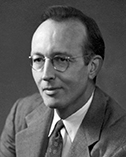
\includegraphics[scale=1]{img/Mac-Lane.eps}
 \captionsetup{labelformat=empty}
 \caption{麦克兰恩(Saunders Mac Lane, 1909 - 2005)}
 \label{fig:Mac-Lane}
\end{wrapfigure}

桑德斯·麦克兰恩1909年生于美国康涅狄格州的诺维奇市。麦克兰恩受洗时的名字是“雷斯利·桑德斯·麦克兰恩”。但是他的父母不喜欢这个名字,所以后来就把雷斯利去掉了。麦克兰恩名字的英文本来是MacLane,他的妻子在打字时总是习惯加上一个空格变成Mac Lane,索性后来麦克兰恩就将错就错了。

麦克兰恩在高中时最喜欢化学。他的父亲在这时去世了,只好由祖父来照顾他。1926年,麦克兰恩的一个远房叔叔资助他到耶鲁学习。他的数学老师希尔带领他参加数学竞赛,并且一路过关斩将获得优胜。从此麦克兰恩下定了从事数学的决心。1930年,麦克兰恩从耶鲁毕业,获得了数学和物理学的双学位。毕业前一年,有一次在新泽西召开耶鲁橄榄球队的球迷聚会。麦克兰恩在会上被授予耶鲁优秀毕业成绩奖\cite{Wiki-Mac-Lane}。恰好芝加哥大学的新任校长哈钦斯也在这次聚会中,他鼓励麦克兰恩到芝加哥大学深造。麦克兰恩于是来到了他后来毕生工作的芝加哥大学\footnote{这里有一段小插曲,聚会后不久,哈钦斯就答应给麦克兰恩一笔奖学金。但是麦克兰恩竟然忘记申请研究生课程就直接去了芝加哥大学。当然最后他被获准入学。}。1931年他获得了硕士学位,接着获得了前往世界数学圣地——哥廷根大学进修的机会。麦克兰恩幸运的成为了最后一批前往哥廷根的美国人,不久纳粹德国就开始禁止美国人前来学习。

在哥廷根,麦克兰恩师从大数学家保罗$\cdot$伯奈斯、埃米$\cdot$诺特、赫尔曼$\cdot$外尔。在他即将获得博士学位的前夕,导师伯奈斯因为是犹太人,被纳粹政府赶出了校园,于是只好由外尔接替伯奈斯。1934年麦克兰恩获得了哥廷根数学研究所的博士学位,并返回美国\footnote{取得学位后,麦克兰恩与来自芝加哥的多萝西$\cdot$琼斯结婚,不久后,他们夫妻一起返回了芝加哥。}。

在1944年与1945年,麦克兰恩领导了在第二次世界大战期间有卓越贡献的哥伦比亚大学应用数学小组。麦克兰恩曾任国家科学院与美国哲学会的副主席,美国数学会的主席。在领导美国数学会的其间,他提倡对现代数学教学技巧改进的研习活动。而在1974年至1980年间,他担任了美国政府的科学顾问。于1976年,以他为首的美国数学家访问团访问了中国,考察了当时中国数学学术发展。麦克兰恩于1949年获选为美国国家科学院院士,并在1989年获得美国国家科学奖章。

麦克兰恩的早期研究方向为域论与赋值论。1941年,麦克兰恩在访问密歇根大学时遇到了艾伦伯格。两人开始在代数和拓扑学上进行合作,并结出了累累硕果。1943年,他与艾伦伯格在研究同调代数时一起创立了范畴论。

2005年,麦克兰恩逝世于美国的旧金山。

\section{范畴}

在介绍范畴的定义前,请先努力忘记集合、函数、映射这些概念。我们以后会看到它们在范畴论中的具体解释。

\begin{definition}
一个范畴$\pmb{C}$包括一组对象(Object)\footnote{和编程中的“面向对象”无关。这里指抽象事物。},记为$A, B, C, ...$,和一组箭头(Arrow),记为$f, g, h, ...$。它们之上定义了以下四种操作:
\begin{itemize}
\item 两个全操作\footnote{全操作(total operation)是指对于所有的对象,无一例外都存在这一操作。与之相对的是部分操作(partial operation),对于某些对象,这一操作没有定义。例如对于全体整数的集合,取相反数$x \mapsto -x$是全操作,而取倒数$x \mapsto 1/x$由于对0没有定义,所以是部分操作。},称为源(source)和目标(target)\footnote{不应把源和目标理解为名词,而应理解为动词。表示“指定源为……”,“指定目标为……”},这两个操作都将对象指定到箭头上记为$A \arrowto{f} B$,表示箭头$f$的源是$A$,目标是$B$;
\item 第三个全操作叫恒等箭头\footnote{同样这里恒等箭头(identity arrow)应理解为动词,表示“为……指定恒等箭头”。},对于任何物体$A$,恒等箭头都指向$A$自己。记为:$A \arrowto{id_A} A$;
\item 第四个操作是一个部分操作,称为组合。它将两个箭头组合起来。如果有箭头$B \arrowto{f} C$和$A \arrowto{g} B$,则$f$和$g$的组合为$f \circ g$,读作“$g$然后$f$”。它表示$A \arrowto{f \circ g} C$。
\end{itemize}

有时我们也将箭头$A \arrowto{f} B$写成$f: A \to B$,如果上下文中对象很清楚,不会产生歧义,有时也直接简写成$f$。如果将对象简记为$Obj$,箭头简记为$Arw$,则组合操作的类型为$(\circ) : Arw \times Arw \to Arw$,表示从两个箭头产生一个新的箭头;源的类型为$src: Arw \to Obj$,表示给某一箭头指定源;目标的类型为$trg: Arw \to Obj$,表示给某一箭头指定目标;恒等箭头的类型为$id: Obj \to Arw$,表示给某一对象指定恒等箭头。

除此之外,范畴还必须满足以下两条公理:

\begin{itemize}
\item \textbf{结合性公理}:箭头组合是可结合的。对任何三个可组合的箭头$f, g, h$都有:
\[
f \circ (g \circ h) = (f \circ g) \circ h
\]
我们可以将其写为$f g h$。
\item \textbf{单位元公理}:恒等箭头对于组合运算来说相当于单位元。
对于任何箭头$A \arrowto{f} B$来说,都有:
\[
f \circ id_A = f = id_B \circ f
\]
\end{itemize}
\end{definition}

由于恒等箭头相当于单位元,我们有时也把$id_A$写成$1_A$,这样组合操作用点“$\circ$”表示,我们可以把它类比为“乘法”。下面的图有助于我们理解单位元公理:

\[
A \arrowto{id_A} A \arrowto{f} B \arrowto{id_B} B
\]

我们再看一下箭头的组合。考虑如下图的3个箭头$f, g, h$,它们组成一个三角形。

\begin{center}
\begin{tikzpicture}
  \matrix (m) [matrix of math nodes,
               row sep=3em, column sep=4em, minimum width=2em]{
     & B & \\
     A & & C \\};
  \path[-stealth]
    (m-2-1) edge node [above] {$f$} (m-1-2)
    (m-1-2) edge node [above] {$g$} (m-2-3)
    (m-2-1) edge node [below] {$h$} (m-2-3);
\end{tikzpicture}
\end{center}

可以沿着两条通路从$A$到达$C$,一条是箭头组合$g \circ f$,另一条是箭头$h$。这样我们就相当于得到了一对平行的箭头:

\begin{center}
\begin{tikzpicture}
  \matrix (m) [matrix of math nodes,
               row sep=3em, column sep=4em, minimum width=2em]{
     A & C\\};
  \path[-stealth]
    (m-1-1.north east) edge node [above] {$g \circ f$} (m-1-2.north west)
    (m-1-1.south east) edge node [below] {$h$} (m-1-2.south west);
\end{tikzpicture}
\end{center}

这两个平行的箭头可能相同,也可能不同。如果它们满足:

\[
h = g \circ f
\]

我们说这个三角形是可交换的(commute),我们后面将大量用到这个概念。

\subsection{范畴的例子}

我们需要用具体的例子来帮助理解范畴这一抽象概念。同时,前面使用的三角形图像能够帮助我们形成直观的感觉。我们会借助这种图(diagram)来对范畴及其关系进行描述。我们举的第一个例子是幺半群。回顾一下上一章中关于幺半群的定义。幺半群可以说是带有单位元的半群。而半群是二元运算满足结合律的集合。例如字符串在连接操作下构成一个幺半群,单位元是空串。

\begin{lstlisting}
instance Monoid String where
    e = ""
    (*) = (++)
\end{lstlisting}

我们可以把字符串幺半群记为$(S, \doubleplus, \texttt{""})$,不难验证它满足幺半群的条件:

\[
\begin{array}{rcl}
r \doubleplus (s \doubleplus t) = (r \doubleplus s) \doubleplus t &
\text{和} &
\texttt{""} \doubleplus s = s = s \doubleplus \texttt{""}
\end{array}
\]

我们再考虑另一个幺半群,群元素是若干个不同字符组成的集合,二元操作是集合的并,单位元是空集。记为$(C, \cup, \{\})$,将两个字符集并在一起可以获得一个更大的字符集,例如:

\[
\{a, b, c, 1, 2\} \cup \{X, Y, Z, 0, 1\} = \{a, b, c, X, Y, Z, 0, 1, 2\}
\]

我们再观察第三个幺半群,集合是包括0的自然数,二元运算是普通加法,单位元是0。记为$(N, +, 0)$。接下来我们建立这三个幺半群之间的态射(morphism),首先是从字符串幺半群$S$到字符集幺半群$C$之间的态射。任给一个字符串,我们可以把串中用到的字符组成一个字符集:

\[
S \arrowto{\phi} C \quad \quad \phi: s \mapsto \{c | c \in s\}
\]

可以验证,这个态射满足以下条件,对于任意两个字符串$r, s$,有:

\[
\begin{array}{rcl}
\phi(s \doubleplus r) = \phi(s) \cup \phi(r) & \text{和} & \phi(\texttt{""}) = \{\}
\end{array}
\]

如果我们把二元运算统一用点“$\circ$”来表示,单位元统一表示为1,则可以写成:

\[
\begin{array}{rcl}
\phi(s \circ r) = \phi(s) \circ \phi(r) & \text{和} & \phi(1) = 1
\end{array}
\]

接下来再定义从字符集$C$到自然数$N$之间的态射。任给一个字符集,我们可以将集合的大小映射为正整数,空集的大小映射为0。

\[
C \arrowto{\psi} N \quad \quad \psi: c \mapsto |c|
\]

有了这两个态射$\phi, \psi$后,我们检查一下它们的组合:

\[
S \arrowto{\phi} C \arrowto{\psi} N
\]

和

\[
S \arrowto{\psi \circ \phi} N
\]

显然组合后$\psi \circ \phi$也是一个态射。这样,我们就得到了幺半群范畴,记为$\pmb{Mon}$。其中对象是幺半群,箭头是态射。恒等箭头是从一个幺半群到它自己的态射:

\[
S \arrowto{id_R} S
\]

注意范畴$\pmb{Mon}$是包含\textbf{所有}幺半群的范畴。这是一个非常巨大的范畴。另一方面,范畴也可以很小,我们接下来看的例子只含有一个幺半群。考虑$(S, \doubleplus, \texttt{""})$,它只有一个对象,就是全体字符串的集合$S$。对于任何字符串$a$,我们都可以定义前缀映射$S \arrowto{(a \doubleplus)} S$:

\[
(a \doubleplus )(x) = a \doubleplus x
\]

这样,箭头$f = (\texttt{"hello"} \doubleplus)$,就会将字符换\texttt{"hello"}添加到任何字符串的前面,例如$f(\texttt{"Alice"})=\texttt{"helloAlice"}$。而箭头$g = (\texttt{"hi"} \doubleplus)$,它可以在任何字符串前添加前缀\texttt{"hi"}\footnote{类似地,还可以定义后缀映射$(\doubleplus b)$。例如箭头$h = (\doubleplus \texttt{"bye"})$在任何字符串后添加后缀\texttt{"bye"}。}。箭头组合$f \circ g$的含义为:

\[
\begin{array}{rl}
(f \circ g)(x) & = f(g(x)) \\
               & = \texttt{"hello"} \doubleplus (\texttt{"hi"} \doubleplus x) \\
               & = (\texttt{"hello"} \doubleplus \texttt{"hi"}) \doubleplus x) \\
               & = \texttt{"hellohi"} \doubleplus x
\end{array}
\]

表示先增加前缀\text{"hi"},然后再增加前缀\texttt{"hello"}。不难验证,任意三个这样的箭头满足结合律。接下来我们还需要检查一下单位元,也就是空串\texttt{""}。以空串作为前缀等于恒等变换:

\[
id(x) = \texttt{""} \doubleplus x = x
\]

这样我们就得到了只有一个对象的幺半群范畴,如图\ref{fig:monoid-as-category}所示。

\begin{figure}[htbp]
\centering
\begin{tikzpicture}
\filldraw (0, 0) circle (4pt) node (obj) {};
\draw[->] (-0.2, 0) arc[radius=5mm, start angle=225, end angle=-45] node[pos=0.5, above]{$f$};
\draw[->] (-0.4, 0) arc[radius=10mm, start angle=225, end angle=-45] node[pos=0.5, above]{$g$};
\draw[->] (-0.6, 0) arc[radius=15mm, start angle=225, end angle=-45] node[pos=0.5, above]{$f \circ g$};
\end{tikzpicture}
\caption{只有一个对象的幺半群范畴}
\label{fig:monoid-as-category}
\end{figure}

同样是幺半群,我们既看到了包含全部幺半群的范畴$\pmb{Mon}$,也看到了只包含一个幺半群的范畴。可谓一沙一世界。更有意思的是,对于任何范畴$\pmb{C}$,和其中任何的对象$a \in \pmb{C}$,定义集合$hom(a, a)$为所有从$a$指向$a$的箭头。则这一箭头的集合在组合运算下又构成一个幺半群,其中单位元是恒等箭头。这种对偶值得我们仔细体会。

类似地,群构成的范畴也有这样特点。有一个由所有群构成的巨大范畴$\pmb{Grp}$,同样每个单个的群$G$本身也构成一个范畴。前者的对象是所有的群,箭头是态射;后者只有一个对象,和幺半群比起来,群中的二元运算都有逆,所以所有的箭头都存在一个逆向的箭头。

我们举的第二个例子是集合。我们让每个集合都成为一个对象\footnote{一旦开始考虑全部集合的集合,就会对导致“全部不包括自身的集合”这样的矛盾,称之为罗素悖论。我们将在第7章详细讲述罗素悖论。},而箭头是从一个集合$A$到另一个集合$B$的函数(或映射)。我们称$A$为函数的定义域,$B$为值域\footnote{确切地说是全函数,即定义域中的每个元素都可以应用的函数}。组合运算就是函数的组合。即$y = f(x)$与$z = g(y)$的组合为$z = (g \circ f)(x) = g(f(x))$。不难验证,函数的组合满足结合律,单位元是恒等函数$id(x) = x$。这样我们就获得了全体集合和函数组成的范畴$\pmb{Set}$。

我们举的第三个例子包括一对概念。分别叫做\textbf{偏序集}和\textbf{预序集}。给定一个集合,所谓预序(pre-order),是说集合中的两个元素之间可以进行比较。我们用抽象的二元关系符号$\leq$来表示,注意这个符号不一定是大于小于关系,它可能表示一个集合是另一个集合的子集,一个字符串是另一个字符串的后缀,一个人是另一个人的后代等等。如果关系$\leq$满足以下两条性质,我们说这是一个预序关系:

\begin{itemize}
\item \textbf{自反性}:任何集合中的元素$a$都有$a \leq a$;
\item \textbf{传递性}:若$a \leq b$且$b \leq c$,则$a \leq c$;
\end{itemize}

如果在此基础上还满足反对称性,则这一关系叫做偏序(partial order):

\begin{itemize}
\item \textbf{反对称性}:若$a \leq b$且$b \leq a$,则$a = b$;
\end{itemize}

我们称满足预序关系的集合叫做预序集,满足偏序关系的集合叫做偏序集,分别记作:

\[
preset \quad \quad \quad poset
\]

\begin{figure}[htbp]
\centering
\begin{tikzpicture}[scale=0.5]
  \matrix (m) [matrix of math nodes,
               row sep=1em, column sep=1em, minimum width=2em]{
     & \text{贾演}   & & & & & \text{贾源} & & \\
     & \text{贾代化} & & & & & \text{贾代善} & & \\
     & \text{贾敬}   & & \text{贾赦} & & \text{贾政} & & & \text{贾敏} \\
     \text{贾珍} & \text{贾惜春} & \text{贾迎春} & \text{贾琏} & \text{贾珠} & \text{贾元春} & \text{贾宝玉} & \text{贾探春} & \text{贾环} \\
     \text{贾蓉} & & & \text{巧姐} & \text{贾兰} & & & & & \\};
  \path[<-]
    (m-1-2) edge (m-2-2) %贾演 -- 贾代化
    (m-1-7) edge (m-2-7) %贾源 -- 贾代善
    (m-2-2) edge (m-3-2) %贾代化 -- 贾敬
    (m-2-7) edge (m-3-4) %--贾赦
    (m-2-7) edge (m-3-6) %--贾政
    (m-2-7) edge (m-3-9) %--贾敏
    (m-3-2) edge (m-4-1) %贾敬--贾珍
    (m-3-2) edge (m-4-2) %贾敬--贾惜春
    (m-3-4) edge (m-4-3) %贾赦--贾迎春
    (m-3-4) edge (m-4-4) %贾赦--贾琏
    (m-3-6) edge (m-4-5) %贾政--贾珠
    (m-3-6) edge (m-4-6) %贾政--贾元春
    (m-3-6) edge (m-4-7) %贾政--贾宝玉
    (m-3-6) edge (m-4-8) %贾政--贾探春
    (m-3-6) edge (m-4-9) %贾政--贾环
    (m-4-1) edge (m-5-1) %贾珍--贾蓉
    (m-4-4) edge (m-5-4) %贾琏--巧姐
    (m-4-5) edge (m-5-5); %贾珠--贾兰
\end{tikzpicture}
\caption{《红楼梦》贾家的家族树}
\label{fig:genealogical-tree}
\end{figure}

在偏序集中,并非任何两个元素都能够进行比较。例如,《红楼梦》中贾家按照祖先关系构成一个偏序集。如果\ref{fig:genealogical-tree}所示。可以看到巧姐$\leq$贾琏,但是贾宝玉和贾探春之间,贾迎春和贾惜春之间无法用$\leq$进行比较。在这棵家族树中,尽管任何人都有祖先(位于树根的人根据自反性,可以认为自己是自己的祖先),但是平辈的人之间无法进行比较。不同枝干上的人之间也无法进行比较。

如图\ref{fig:powerset}所示,一个集合$\{x, y, z\}$的所有子集在包含关系下构成一个偏序集。尽管图中任意元素,都可以找到其子集,但是图中同一层级上的元素间无法比较,另外$\{x\}$和$\{y, z\}$间也无法比较。

\begin{figure}[htbp]
 \centering
 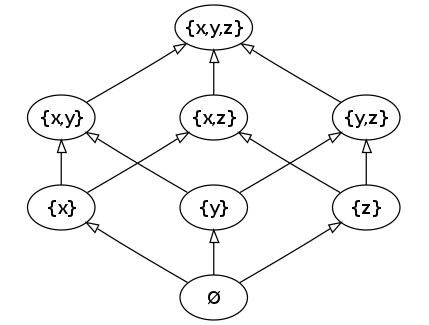
\includegraphics[scale=0.4]{img/powerset.eps}
 %\captionsetup{labelformat=empty}
 \caption{一个集合的子集在包含关系下构成一个偏序集}
 \label{fig:powerset}
\end{figure}

一般来说,任何一个偏序集都是一个预序集,但是反过来却不一定成立。一个预序集不一定是一个偏序集。考虑带有偏序(或者预序)关系的两个集合$(R, \leq)$和$(S, \leq)$。一个单调映射

\[
R \arrowto{f} S
\]

是满足如下条件的函数。对于$R$中的任意两个元素$x, y$

\[
\text{若} x \leq y \text{,则} f(x) \leq f(y)
\]

不难验证,对于任意两个单调映射:

\[
R \arrowto{f} S \arrowto{g} T
\]

它们的组合$g \circ f$也是单调函数。这样我们就获得了一对范畴

\[
\pmb{Pre} \quad \quad \quad \pmb{Pos}
\]

它们的对象分别是所有的$preset$和$poset$,两个范畴中的箭头都是单调映射。由于恒等映射也是单调映射,所以范畴中的恒等箭头为恒等映射。

考虑一对偏序集$R, S$,由于每个偏序集也是预序集,所以下面两个集合——所有从$R$出发到$S$的箭头组成的集合——是相等的。

\[
\pmb{Pre}[R, S] \quad \quad \quad \pmb{Pos}[R, S]
\]

这是因为,箭头集合中的每个元素都是一个从$R$到$S$的单调函数。这说明$\pmb{Pos}$是$\pmb{Pre}$的\textbf{子范畴}。

幺半群范畴和预序集范畴这两个例子不是随便挑选的,我们有着特殊的用意。这两个范畴可以说是最简单的例子。通过幺半群范畴,我们可以学习组合;通过预序集范畴,我们可以学习比较。对数学结构的组合与比较是整个范畴论的核心。在这一意义上,任何范畴都是幺半群与预序集的某种混合形式\cite{Simmons2011}。

$\pmb{Pre}$是包含所有预序集的巨大范畴。另一方面预序集范畴也可以很小。小到只含有一个预序集。其中的对象是预序集$(S, \leq)$中的元素$i, j, k, ...$。对于可比较的对象$i, j$,如果$i \leq j$,我们就定义箭头

\[
i \longrightarrow j
\]

这样任何对象间或者没有箭头,表示它们不可比较;或者存在一个箭头,表示它们有$\leq$关系。总之,任何两个对象间最多只有一个箭头。为了方便有时我们在箭头行做如下标记:

\[
i \arrowto{(j, i)} j
\]

看起来,似乎用$(j, i)$表示$i \leq j$像是写反了,格外别扭。实际上它会带来表达上的好处。我们来检验一下箭头的单位元和组合:

\[
\begin{array}{rll}
id_i & = (i, i) & \text{因为:} i \leq i \\
(k, j) \circ (j, i) & = (k, i) & \text{若} i \leq j \leq k \text{,则} i \leq k
\end{array}
\]

这样的确一个预序集就是一个范畴。我们再次看到了预序集范畴和幺半群范畴的对偶。幺半群作为范畴只含有一个对象,却含有丰富的箭头;预序集作为范畴对象很多,但是对象间的箭头却最多只有一个。

\begin{Exercise}
\Question{验证幺半群$(C, \cup, \{\})$和$(N, +, 0)$都是只含有一个对象的范畴。}
\Question{第一章中我们介绍了自然数的皮亚诺公理,并且介绍了和皮亚诺算术同构的其它结构,例如链表等。这些完全可以用范畴来解释。这一结论是德国数学家戴德金发现的,尽管当时还没有范畴论。我们今天将这一范畴命名为皮亚诺范畴$\pmb{Pno}$。范畴中的对象为$(A, f, z)$,其中$A$为元素的集合,对于自然数来说这个集合是全体自然数$N$;$f: A \to A$是后继函数,对于自然数来说,就是$succ$;$z \in A$是起始元素,对于自然数来说是0。任给两个皮亚诺对象$(A, f, z)$和$(B, g, c)$,现在定义态射
\[
A \arrowto{\phi} B
\]
它满足

\[
\phi \circ f = g \circ \phi \quad \text{且} \quad \phi(z) = c
\]

试验证$\pmb{Pno}$的确是一个范畴。}
\end{Exercise}

\subsection{箭头$\neq$函数}

在此前的例子中,箭头要么是一般意义上的函数,要么是类似函数意义的映射和态射。这容易造成一种错觉,认为箭头等同于函数。我们接下来看的例子有助于打破这种错觉。

\begin{example}
在这个例子中,对象是有限集合。箭头仍然是函数,但是意义变了。若集合$A$到集合$B$间有一个箭头$f$为$A \arrowto{f} B$。但是$f$的意义是这样一个函数$f: A \times B \to \mathbb{R}$,也就是说$f$接受两个自变量,分别是$A$和$B$中的元素,然后得到一个实数。如果从$B$到$C$还有一个这样的箭头$g$,其意义为:$g: B \times C \to \mathbb{R}$,则箭头的组合

\[
A \arrowto{f} B \arrowto{g} C
\]

组合的意义为:$g \circ f : A \times C \to \mathbb{R}$

这个组合函数的效果是怎样的呢?我们定义:

\[
(g \circ f)(a, c) = \sum\{f(a, x) g(x, c) | x \in B\}
\]

也就是说,我们从中间集合$B$中依次拿出每个元素$x$,计算$f(a, x)$和$g(x, c)$的积,然后将结果累加起来。显然这还是一个实数。不难验证,这构成一个范畴。
\end{example}

\begin{example}
接下来的例子名叫关系范畴$\pmb{Rel}$。范畴中的对象是集合。从对象$A$到$B$的箭头$A \arrowto{R} B$的定义为:

\[
R \subseteq B \times A
\]

我们来看看这个箭头的含义是什么。集合$B \times A$代表了所有$B$和$A$中元素对的组合。也叫做$B$和$A$的积:

\[
B \times A = \{(b, a) | a \in A, b \in B\}
\]

我们以红楼梦人物为例,集合$A =$ \{贾蓉, 贾惜春, 贾琏\},集合$B =$ \{秦可卿, 王熙凤\},则$B \times A$的积为\{(秦可卿, 贾蓉), (秦可卿, 贾惜春), (秦可卿, 贾琏), (王熙凤, 贾蓉), (王熙凤, 贾惜春), (王熙凤, 贾琏)\}。集合$R$是$B \times A$的子集,它可以看作$A$与$B$的某种关系。如果$A$中的元素$a$和$B$中的元素$b$满足关系$R$,则有$(b, a) \in R$,我们将其记为$bRa$。具体到这个例子,我们令$R=$\{(秦可卿, 贾蓉), (王熙凤, 贾琏)\},则$R$代表婚姻关系。

这样从对象$A$到$B$的\textbf{所有}箭头构成的集合$\pmb{Rel}[A, B]$就代表了从$A$到$B$的各种可能的关系。现在我们考虑箭头的组合

\[
A \arrowto{R} B \arrowto{S} C
\]

定义箭头组合$S \circ R$为:

\[
c (S \circ R) a \iff \exists b \in B \text{使得} cSbRa
\]

也就是说,存在某个中间集合中的元素$b$,同时使得两个关系$bRa$,$cSb$都成立。即$(b, a) \in R$且$(c, b) \in S$。

具体到红楼梦的例子,令集合$C=$\{王夫人, 薛姨妈, 邢夫人\},关系$S=$\{(王夫人, 王熙凤), (薛姨妈, 王熙凤)\}表示姑妈关系。这样组合箭头$S \circ R$的结果是:\{(王夫人, 贾琏), (薛姨妈, 贾琏)\},表示$c$的侄女嫁给了$b$的关系。也就是说王夫人、薛姨妈和贾琏都通过王熙凤使得两个关系同时成立。

恒等箭头的定义很简单为:

\[
id_A = \{(a, a) | a \in A\}
\]

表示所有元素都和自己产生恒等关系。
\end{example}

我们还可以从任何已知的范畴产生新的范畴,例如把一个范畴$\pmb{C}$中的所有箭头反向就得到了一个对偶的范畴$\pmb{C}^{op}$。这样我们了解了一个范畴,就同时了解了它的对偶范畴。

\begin{Exercise}
\Question{本节第一例子中的恒等箭头是什么?}
\Question{考虑集合上的部分函数构成的范畴$\pmb{Pfn}$。对象是集合,而箭头是部分函数,从集合$A$的$B$的部分函数$A \arrowto{f} B$是说,对于$A$的子集$A'$来说$f$有定义。这个范畴中的箭头组合、单位箭头的含义是什么?}
\end{Exercise}

\subsection{左右消去}

范畴中的某些箭头具有有一些特殊的性质,我们这一节介绍一对相对偶的性质,称为左消去\footnote{也有人译为“首一”,但是这里译为消去更易理解。}(monic)和右消去(epic)。既然是对偶的性质,我们就用对偶的形式给出:

\begin{definition}
如果范畴中的箭头
\[
B \arrowto{m} A \quad \quad \quad A \arrowto{e} B
\]
对任意一对平行的箭头

\begin{center}
\begin{tikzpicture}
  \matrix (m) [matrix of math nodes,
               row sep=3em, column sep=4em, minimum width=2em]{
     X & B & & B & X\\};
  \path[-stealth]
    (m-1-1.north east) edge node [above] {$f$} (m-1-2.north west)
    (m-1-1.south east) edge node [below] {$g$} (m-1-2.south west)
    (m-1-4.north east) edge node [above] {$f$} (m-1-5.north west)
    (m-1-4.south east) edge node [below] {$g$} (m-1-5.south west);
\end{tikzpicture}
\end{center}

均满足如下条件:

\[
\text{若} m \circ f = m \circ g \text{,则}f = g \quad \quad \quad
\text{若} f \circ e = g \circ e \text{,则}f = g
\]

我们称$m$为可\textbf{左消去}的,$e$为可\textbf{右消去}的。
\end{definition}

左右可消去箭头有一些有趣的性质,我们以左消去为例,读者可以尝试用对偶的方式思考右消去的情形。如果两个箭头是左消去的,则它们的组合也是左消去的。

\begin{proof}
令$m: A \to B$和$n: B \to C$都是左消去的,若$(n \circ m) \circ f = (n \circ m) \circ g$,我们有

\[
\begin{array}{rll}
(n \circ m) \circ f & = (n \circ m) \circ g & \\
n \circ (m \circ f) & = n \circ (m \circ g) & \text{结合律} \\
m \circ f &= m \circ g & \text{因为$n$是左消去的} \\
f & = g & \text{因为$m$是左消去的}
\end{array}
\]
所以,组合$m \circ n$也是左消去的。
\end{proof}

\begin{Exercise}
\Question{证明右消去箭头的组合也是右消去的。}
\end{Exercise}

\section{函子}

\section{自然变换}

\section{积和余积}

\subsection{起始对象和终止对象}

\section{数据类型}

\section{伴随}

\ifx\wholebook\relax \else
\begin{thebibliography}{99}

\bibitem{Dieudonne1987}
[法]让$\cdot$迪厄多内 著,沈用欢 译 ``当代数学,为了人类心智的荣耀''. 上海教育出版社. 2000年3月. ISBN: 7532063062

\bibitem{Monad-Haskell-Wiki}
Haskell Wiki. ``Monad''. \url{https://wiki.haskell.org/Monad}

\bibitem{Wiki-Eilenberg}
Wikipedia. ``塞缪尔$\cdot$艾伦伯格''. \url{https://en.wikipedia.org/wiki/Samuel_Eilenberg}

\bibitem{Wiki-Mac-Lane}
Wikipedia. ``桑德斯$\cdot$麦克兰恩''. \url{https://en.wikipedia.org/wiki/Saunders_Mac_Lane}

\bibitem{Simmons2011}

Harold Simmons. ``An introduction to Category Theory''.  Cambridge University Press; 1 edition, 2011. ISBN: 9780521283045

\end{thebibliography}

\expandafter\enddocument
%\end{document}

\fi
